\documentclass[12pt,twoside]{article}

\textwidth 17cm \textheight 25cm \evensidemargin 0cm
\oddsidemargin 0cm \topmargin -2cm
\parindent 0pt
%\parskip \bigskipamount

\usepackage{graphicx}
\usepackage[dutch]{babel}
\usepackage{amssymb,amsthm,amsmath}
%\usepackage{dot2texi}
\usepackage[utf8]{inputenc}
\usepackage{nopageno}
\usepackage{pdfpages}
\usepackage{enumerate}
\usepackage{caption}
\usepackage{wrapfig}
\usepackage{pgf,tikz,pgfplots}
\pgfplotsset{compat=1.15}
\usepackage{color}
\usetikzlibrary{arrows}
\usetikzlibrary{patterns}
\usepackage{fancyhdr}
\pagestyle{fancy}
\usepackage[version=3]{mhchem}
\usepackage{multicol}
\usepackage{fix-cm}
\usepackage{setspace}
\usepackage{mhchem}
\usepackage{xhfill}
\usepackage{parskip}
\usepackage{cancel}
\usepackage{mdframed}
\usepackage{url}
\usepackage{mathtools}
\usepackage{changepage}

\newcommand{\todo}[1]{{\color{red} TODO: #1}}

\newcommand{\degree}{\ensuremath{^\circ}}
\newcommand\rad{\qopname\relax o{\mathrm{rad}}}

\newcommand\ggd{\qopname\relax o{\mathrm{ggd}}}

\pgfmathdeclarefunction{gauss}{2}{%
  \pgfmathparse{1/(#2*sqrt(2*pi))*exp(-((x-#1)^2)/(2*#2^2))}%
}

\def\LRA{\Leftrightarrow}

\newcommand{\zrmbox}{\framebox{\phantom{EXE}}\phantom{X}}
\newcommand{\zrm}[1]{\framebox{#1}}

% environment oefening:
% houdt een teller bij die de oefeningen nummert, probeert ook de oefening op één pagina te houden
\newcounter{noefening}
\setcounter{noefening}{0}
\newenvironment{oefening}
{
  \stepcounter{noefening}
  \pagebreak[0]
  \begin{minipage}{\textwidth}
  \vspace*{0.7cm}{\large\bf Oefening \arabic{noefening}}
}{%
  \end{minipage}
}

\usepackage{calc}

% vraag
\reversemarginpar
\newcounter{punten}
\setcounter{punten}{0}
\newcounter{nvraag}
\setcounter{nvraag}{1}
\newlength{\puntwidth}
\newlength{\boxwidth}
\newcommand{\vraag}[1]{
\settowidth{\puntwidth}{\Large{#1}}
\setlength{\boxwidth}{1.5cm}
\addtolength{\boxwidth}{-\puntwidth}
{\large\bf Vraag \arabic{nvraag} \addtocounter{nvraag}{1}}\vspace*{-0.5cm}
{\marginpar{\color{lightgray}\fbox{\parbox{1.5cm}{\vspace*{1cm}\hspace*{\boxwidth}{\Large{#1}}}}}
\vspace*{0.5cm}}
\addtocounter{punten}{#1}}

% arulefill
\def\arulefill{\leavevmode{\xrfill[-5pt]{0.3pt}[lightgray]\endgraf}\vspace*{0.2cm}}

% \arules{n}
\newcommand{\arules}[1]{
\color{lightgray}
%\vspace*{0.05cm}
\foreach \n in {1,...,#1}{
  \vspace*{0.75cm}
  \hrule height 0.3pt\hfill
}\color{black}\vspace*{0.2cm}}

% \arule{x}
\newcommand{\arule}[1]{
\color{lightgray}{\raisebox{-0.1cm}{\rule[-0.05cm]{#1}{0.3pt}}}\color{black}
}

% \abox{y}
\newcommand{\abox}[1]{
\fbox{
\begin{minipage}{\textwidth- 4\fboxsep}
\hspace*{\textwidth}\vspace{#1}
\end{minipage}
}
}

\newcommand{\ruitjes}[1]{
\definecolor{cqcqcq}{rgb}{0.85,0.85,0.85}
\hspace*{-2.5cm}
\begin{tikzpicture}[scale=1.04,line cap=round,line join=round,>=triangle 45,x=1.0cm,y=1.0cm]
\draw [color=cqcqcq, xstep=0.5cm, ystep=0.5cm] (0,-#1) grid (20.5,0);
\end{tikzpicture}
}


\newcommand{\assenstelsel}[5][1]{
\definecolor{cqcqcq}{rgb}{0.65,0.65,0.65}
\begin{tikzpicture}[line cap=round,line join=round,>=triangle 45,x=#1cm,y=#1cm]
\draw [color=cqcqcq,dash pattern=on 1pt off 1pt, xstep=1.0cm,ystep=1.0cm] (#2,#4) grid (#3,#5);
\draw[->,color=black] (#2,0) -- (#3,0);
%\draw[shift={(1,0)},color=black] (0pt,2pt) -- (0pt,-2pt) node[below] {\footnotesize $1$};
%\draw[color=black] (#3.25,0.07) node [anchor=south west] {$x$};
\draw[->,color=black] (0,#4) -- (0,#5);
%\draw[shift={(0,1)},color=black] (2pt,0pt) -- (-2pt,0pt) node[left] {\footnotesize $1$};
\draw[color=black] (0.09,#5.25) node [anchor=west] {\phantom{$y$}};
%\draw[color=black] (0pt,-10pt) node[right] {\footnotesize $0$};
\end{tikzpicture}
}

\newcommand{\getallenas}[3][1]{
\definecolor{cqcqcq}{rgb}{0.65,0.65,0.65}
\begin{tikzpicture}[scale=#1,line cap=round,line join=round,>=triangle 45,x=1.0cm,y=1.0cm]
\draw [color=cqcqcq,dash pattern=on 1pt off 1pt, xstep=1.0cm,ystep=1.0cm] (#2,-0.2) grid (#3,0.2);
\draw[->,color=black] (#2.25,0) -- (#3.5,0);
\draw[shift={(0,0)},color=black] (0pt,2pt) -- (0pt,-2pt) node[below] {\footnotesize $0$};
\draw[shift={(1,0)},color=black] (0pt,2pt) -- (0pt,-2pt) node[below] {\footnotesize $1$};
\draw[color=black] (#3.25,0.07) node [anchor=south west] {$\mathbb{R}$};
\end{tikzpicture}
}

\newcommand{\visgraad}[1]{\begin{tabular}{p{0.5cm}|p{#1}}&\\\hline\\\end{tabular}}

\newcommand{\tekenschema}[2]{\begin{tabular}{p{0.5cm}|p{#1}}&\\\hline\\[#2]\end{tabular}}

% schema van Horner
\newcommand{\schemahorner}{
\begin{tabular}{p{0.5cm}|p{7cm}}
&\\[1.5cm]
\hline\\
\end{tabular}}

% geef tabular iets meer ruimte
\setlength{\tabcolsep}{14pt}
\renewcommand{\arraystretch}{1.5}

\newcommand{\toets}[3]{
\thispagestyle{plain}
\vspace*{-2.5cm}
\begin{tikzpicture}[remember picture, overlay]
    \node [shift={(15.25 cm,-1.6cm)}] {%
        \includegraphics[width=1.8cm]{/home/ppareit/kaa1415/logokaavelgem.png}%
    };%
\end{tikzpicture}

\begin{tabular}{|llc|c|}
\hline
\vspace*{-0.5cm}
&&&\\
Naam & \arule{4cm} & {\Large\bf KA AVELGEM} & \\
\vspace*{-0.75cm}
&&&\\
Klas & \arule{4cm} & {\Large\bf 20...-...-...} & \\
\hline
\vspace*{-0.75cm}
&&&\\
Toets & {\bf #2} & {\large\bf #1} & Beoordeling\\
\vspace*{-0.75cm}
&&&\\
Onderwerp & \multicolumn{2}{l|}{\bf #3} &\\
\hline
\end{tabular}
}

\newcommand{\oefeningen}[1]{

\fancyhead[LE, RO]{\vspace{0.5cm} #1}
%\thispagestyle{plain}

{\bf \Large \centering Oefeningen: #1}

}

\raggedbottom

\newcommand\vl{\qopname\relax o{\mathrm{vl}}}

\newcommand\dom{\qopname\relax o{\mathrm{dom}}}
\newcommand\ber{\qopname\relax o{\mathrm{ber}}}

\newcommand\mC{\qopname\relax o{\mathrm{mC}}}
\newcommand\uC{\qopname\relax o{\mathrm{{\mu}C}}}
\newcommand\C{\qopname\relax o{\mathrm{C}}}

\newcommand\W{\qopname\relax o{\mathrm{W}}}
\newcommand\kW{\qopname\relax o{\mathrm{kW}}}
\newcommand\kWh{\qopname\relax o{\mathrm{kWh}}}


\newcommand\V{\qopname\relax o{\mathrm{V}}}
\newcommand\ohm{\qopname\relax o{\mathrm{\Omega}}}
\newcommand\kohm{\qopname\relax o{\mathrm{k\Omega}}}


\newcommand\N{\qopname\relax o{\mathrm{N}}}

\newcommand\Nperkg{\qopname\relax o{\mathrm{N/kg}}}

\newcommand\Nperm{\qopname\relax o{\mathrm{N/m}}}

\newcommand\gpermol{\qopname\relax o{\mathrm{g/mol}}}


\newcommand\kgperm{\qopname\relax o{\mathrm{kg/m}}}
\newcommand\kgperdm{\qopname\relax o{\mathrm{kg/dm}}}
\newcommand\gpercm{\qopname\relax o{\mathrm{g/cm}}}
\newcommand\gperml{\qopname\relax o{\mathrm{g/ml}}}


\newcommand{\mA}{\;\mbox{mA}}
\newcommand{\A}{\;\mbox{A}}
\newcommand{\MA}{\;\mbox{MA}}

\newcommand{\us}{\;\mu\mbox{s}}
\newcommand\s{\qopname\relax o{\mathrm{s}}}

\newcommand\h{\qopname\relax o{\mathrm{h}}}

\newcommand{\kmperh}{\;\mbox{km/h}}
\newcommand{\mpers}{\;\mbox{m/s}}
\newcommand{\kmpermin}{\;\mbox{km/min}}
\newcommand{\kmpers}{\;\mbox{km/s}}

\newcommand{\mph}{\;\mbox{mph}}

\newcommand{\Hz}{\;\mbox{Hz}}

\newcommand\Gm{\qopname\relax o{\mathrm{Gm}}}
\newcommand\Mm{\qopname\relax o{\mathrm{Mm}}}
\newcommand\km{\qopname\relax o{\mathrm{km}}}
\newcommand\hm{\qopname\relax o{\mathrm{hm}}}
\newcommand\dam{\qopname\relax o{\mathrm{dam}}}
\newcommand\m{\qopname\relax o{\mathrm{m}}}
\newcommand\dm{\qopname\relax o{\mathrm{dm}}}
\newcommand\cm{\qopname\relax o{\mathrm{cm}}}
\newcommand\mm{\qopname\relax o{\mathrm{mm}}}
\newcommand\um{\qopname\relax o{\mathrm{{\mu}m}}}
\newcommand\nm{\qopname\relax o{\mathrm{nm}}}


\newcommand\Gg{\qopname\relax o{\mathrm{Gg}}}
\newcommand\Mg{\qopname\relax o{\mathrm{Mg}}}
\newcommand\kg{\qopname\relax o{\mathrm{kg}}}
\newcommand\hg{\qopname\relax o{\mathrm{hg}}}
\renewcommand\dag{\qopname\relax o{\mathrm{dag}}}
\newcommand\g{\qopname\relax o{\mathrm{g}}}
\newcommand\dg{\qopname\relax o{\mathrm{dg}}}
\newcommand\cg{\qopname\relax o{\mathrm{cg}}}
\newcommand\mg{\qopname\relax o{\mathrm{mg}}}
\newcommand\ug{\qopname\relax o{\mathrm{{\mu}g}}}
\renewcommand\ng{\qopname\relax o{\mathrm{ng}}}

\newcommand\ton{\qopname\relax o{\mathrm{ton}}}

\newcommand\Gl{\qopname\relax o{\mathrm{Gl}}}
\newcommand\Ml{\qopname\relax o{\mathrm{Ml}}}
\newcommand\kl{\qopname\relax o{\mathrm{kl}}}
\newcommand\hl{\qopname\relax o{\mathrm{hl}}}
\newcommand\dal{\qopname\relax o{\mathrm{dal}}}
\renewcommand\l{\qopname\relax o{\mathrm{l}}}
\newcommand\dl{\qopname\relax o{\mathrm{dl}}}
\newcommand\cl{\qopname\relax o{\mathrm{cl}}}
\newcommand\ml{\qopname\relax o{\mathrm{ml}}}
\newcommand\ul{\qopname\relax o{\mathrm{{\mu}l}}}
\newcommand\nl{\qopname\relax o{\mathrm{nl}}}

\newcommand\MJ{\qopname\relax o{\mathrm{MJ}}}
\newcommand\kJ{\qopname\relax o{\mathrm{kJ}}}
\newcommand\J{\qopname\relax o{\mathrm{J}}}

\newcommand\T{\qopname\relax o{\mathrm{T}}}
\newcommand\uT{\qopname\relax o{\mathrm{{\mu}T}}}

\newcommand\grC{\qopname\relax o{\mathrm{{\degree}C}}}

\newcommand\K{\qopname\relax o{\mathrm{K}}}
\newcommand\calperK{\qopname\relax o{\mathrm{cal/K}}}

\newcommand\hPa{\qopname\relax o{\mathrm{hPa}}}
\newcommand\Pa{\qopname\relax o{\mathrm{Pa}}}

\newcommand\dB{\qopname\relax o{\mathrm{dB}}}

\newcommand\Var{\qopname\relax o{\mathrm{Var}}}

\newcommand{\EE}[1]{\cdot 10^{#1}}

\onehalfspacing

%\setlength{\headsep}{0cm}

\newenvironment{exlist}[1] %
{ \begin{multicols}{#1}
  \begin{enumerate}[(a)]
    \setlength{\itemsep}{0.5em} }
{ \end{enumerate}
  \end{multicols} }




\usepackage{pgfplots}

\usepackage{relsize}


\usepackage{versions}
\excludeversion{theorie}
%\includeversion{theorie}

\newtheorem{definition}{Definitie}
\newtheorem{eigenschap}{Eigenschap}

% vergelijkingen mooi uitlijnen:
% \begin{alignat}{2}
%   &&    a^2-b^2 &= 0\\
%   \lra && (a-b)(a+b) &= 0\\
% \end{alignat}
\newcommand{\lra}{\ensuremath{\Leftrightarrow\qquad}}



\begin{document}

\pagestyle{fancy}
\lhead{}
\rhead{Oefeningen Veeltermfuncties}

\begin{theorie}
\thispagestyle{empty}
\begin{center}
  \begin{mdframed}
  \centering
  \fontsize{40}{60}\selectfont Veeltermfuncties
  \end{mdframed}
  \vfill
  \vfill
\end{center}

\subsection*{Doelstellingen}
\vspace*{-0.8cm}
{\singlespacing
Je \hfill  {\scriptsize(LP2006-059, LI1.1, ET14)}
\begin{itemize}
\end{itemize}}

\thispagestyle{empty}
\mbox{}
\newpage
\clearpage
\thispagestyle{empty}
%\mbox{}
\tableofcontents
\newpage
\clearpage
\pagenumbering{arabic} 

\fancyhead[RO,LE]{Veeltermfuncties}
\fancyhead[RE,LO]{}

\end{theorie}

\onehalfspacing

\pagebreak

\section{Veeltermvergelijking}

\begin{oefening}
  Los de volgende vergelijkingen van de eerste graad op in $\mathbb{R}$
  \begin{multicols}{2}
    \begin{enumerate}[(a)]
      \itemsep0.7em
    \item $4x-8=0$
    \item $3x+9=0$
    \item $-3x+9=0$
    \item $2(x+6)=4-(x+7)$
    \item $x - \dfrac{x-2}{3} = 4$
    \item $2(x-3)+7=5-(2-x)$
    \item $(x+1)^2-2=x(x-3)-(1-2x)$
    \item $\dfrac{3+2x}{4}-\dfrac{4x-5}{5}=\dfrac{21-6x}{6}$
    \item $\dfrac{4x}{3}-\left(\dfrac{3}{2}-\dfrac{x}{4}\right)=x+4\left(\dfrac{2x}{3}-1\right)$
    \item $\dfrac{3(x-1)}{5}-\dfrac{2(1-4x)}{7}=x+\dfrac{x+1}{5}$
    \item $\dfrac{5x}{8}-\dfrac{x-\frac{5}{2}}{4}=1$
    \item $\dfrac{x}{5}+\dfrac{x}{2}=-7$
    \item $\dfrac{3-x}{4}-\dfrac{x-2}{3}=\dfrac{x}{2}-\dfrac{4x+1}{12}$
    \end{enumerate}
  \end{multicols}
\end{oefening}

\begin{oefening}
  Los de volgende vergelijkingen van de tweede graad op in $\mathbb{R}$
  \begin{multicols}{2}
    \begin{enumerate}[(a)]
      \itemsep0.7em
    \item $2x^2-4x-6=0$
    \item $5x(x-2)=x(3x-4)-5$
    \item $\frac{2}{3}x^2+5x+1=0$
    \item $80x^2+8x=15$
    \item $80x^2+15=-8x$
    \item $(3-x)(3+x)=(x-4)^2$
    \item $(x-2)^2=x^2-4$
    \item $(3x+2)(3x-2)+6x+5=0$
    \item $x+1=(x+1)(x-1)$
    \item $4x^2-20x+25=0$
    \item $3x^2+5=0$
    \item $x=x^2$
    \item $2\left(7x+32\right)=(3x+8)^2$
    \item $11x+13=2x^2$
    \item $x\left(x+3\right)+2\left(5+2x\right)=0$
    \item $x^2+2x-8=0$
    \item $(x+3)^2=16$
    \item $9x^2+30x+25=0$
    \item $10x^2+7x-3=0$
    \item $x^2=x+1$
    \item $37x^2+13x-50=0$
    \item $3x(3x+10)+5=-20$
    \item $x^2=3x-18$
    \item $x^2=10x-25$
    \end{enumerate}
  \end{multicols}
\end{oefening}

\begin{oefening}
  Los op in $\mathbb{R}$
  \begin{enumerate}[(a)]
      \itemsep1em
    \item $x^2+x-8=(x-6)^2$% \tabto{6cm} {\color{gray}$V=\{\dfrac{44}{13}\}$}
    \item $x^2+\dfrac{15}{2}=\dfrac{11x}{2}$% \tabto{6cm} {\color{gray}$V=\{\dfrac{5}{2}, 3\}$}
    \item $(2x-4)(2x+4)=(x+2)^2$% \tabto{6cm} {\color{gray}$V=\{-2,\dfrac{10}{3}\}$}
    \item $9x^2-36=(6+3x)^2$% \tabto{6cm} {\color{gray}$V=\{-2\}$}
    \item $19-x+x^2=18-2x-x^2$% \tabto{6cm} {\color{gray}$V=\{\}$}
    \item $25x^2+20x=-9$% \tabto{6cm} {\color{gray}$V=\{-\dfrac{3}{5}\}$}
    \item $6x^2=x+1$% \tabto{6cm} {\color{gray}$V=\{-\dfrac{1}{3},\dfrac{1}{2}\}$}
  \end{enumerate}
\end{oefening}

\begin{oefening}
De ring links en de cirkel rechts hebben dezelfde oppervlakte. Bepaal $x$.
\begin{center}
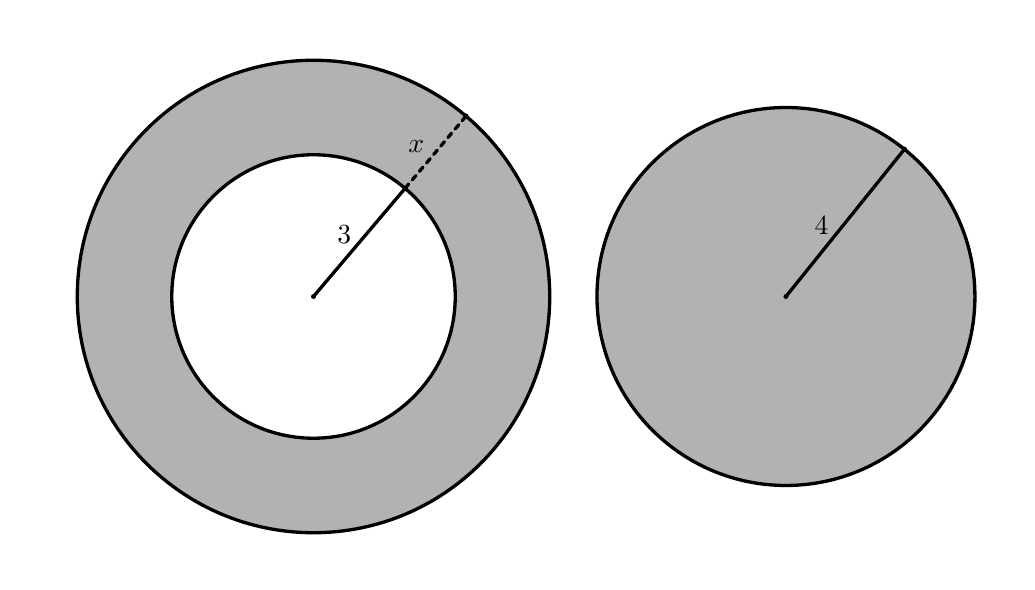
\begin{tikzpicture}[scale=0.6, line cap=round,line join=round,>=triangle 45,x=1.0cm,y=1.0cm]
\clip(-2.05,-0.62) rectangle (18.68,10.69);
\draw [line width=1.2pt,fill=gray!60] (4,5) circle (5cm);
\draw [line width=1.2pt,fill=white] (4,5) circle (3cm);
\draw [line width=1.2pt,fill=gray!60] (14,5) circle (4cm);
\draw [line width=1.2pt] (14,5)-- (16.51,8.12);
\draw [line width=1.2pt] (4,5)-- (5.94,7.29);
\draw [line width=1.2pt,dash pattern=on 2pt off 2pt] (5.94,7.29)-- (7.23,8.82);
\draw (5.8,8.5) node[anchor=north west] {$x$};
\draw (4.3,6.7) node[anchor=north west] {3};
\draw (14.4,6.9) node[anchor=north west] {4};
\fill [color=black] (4,5) circle (1.5pt);
\fill [color=black] (14,5) circle (1.5pt);
\fill [color=black] (7.23,8.82) circle (1.5pt);
\fill [color=black] (16.51,8.12) circle (1.5pt);
\fill [color=black] (5.94,7.29) circle (1.5pt);
\end{tikzpicture}
\end{center}
\end{oefening}

\begin{oefening}
  Los op in $\mathbb{R}$
  \begin{multicols}{2}
    \begin{enumerate}[(a)]
    \itemsep0.7em
    \item $x^3+2x-3=0$
    \item $7x^3+8x^2+3x+2=0$
    \item $x^3-x+6=0$
    \item $3x^2(x-1)=\dfrac{7}{2}x^2-2$
    \item $8x^3+12x^2+6x+2=0$
    \item $20x^3+60x^2+45x=0$
    \item $x^4-4x^3-x^2+16x-12=0$
    \item $x+\dfrac{7x}{2}=\dfrac{3x^3}{2}+\dfrac{3x^2}{2}+\dfrac{3}{2}$
    \item $x^3+(2x+1)^2=x+1$
    \end{enumerate}
  \end{multicols}
\end{oefening}

\begin{oefening} % www3.ul.ie/~mlc/support/.../chap3/3_3.pdf
  Los volgende vergelijkingen van graad hoger dan twee op in $\mathbb{R}$:
  \begin{multicols}{2}
  \begin{enumerate}[(a)]
  \itemsep.7em
  \item $x^3-17x^2+54x-8=0$
  \item $x^3-6x^2+11x-6=0$
  \item $x^3-7x=6$
  \item $2x^3+9x^2+7x+2=2x^2$
  \item $22x+8=3x^3+7x^2$
  \item $2x^4+8x^3-\dfrac{7x^2}{2}-\dfrac{67x}{2}-15=0$
  \item $4x^4+8x^3+3x^2-2x-1=0$
  \end{enumerate}
  \end{multicols}
\end{oefening}

\begin{oefening}
Los op in $\mathbb{R}$:
\begin{enumerate}[(a)]
  \itemsep0.6em
  \begin{multicols}{2}
  \item $2x^3+3x^2-17x+12=0$
  \item $3x^3+13x^2-18x-40=0$
  \item $x^3+4x^2-15x-18=0$
  \item $2x^3+9x^2+7x-6=0$
  \item $-3x^3+16x^2-17x+4=0$
  \item $2x^4+3x^3=17x^2-12x$
  \item $16x^3+4x=3x^4+17x^2$
  \item $2x^4-11x^3-12x^2+36x=0$
  \item $x^4+3x^3-51x^2+37x+90=0$
  \item $6x^3-11x^2-3x+2=0$
  \item $x^3-9x^2+26x=24$
  \item $x^3-3x+2=0$
  \item $x^4+x^3=10x^2-8x$
  \item $x^4+2x-1=2x^3$
  \item $1=x^4$
  \item $3x^2+x(x-1)^2=5x+4$
  \item $(x+1)(x^2+2x+1)=2x(x+2)-1$
  \item $x^3+70=39x$
  \item $x^4+3x^2+10x=6x^3$
  \item $-2(10x+x^3)=x^2(10+x^2)$
  \item $x^4+82x+176=93x^2-2x^3$
  \item $12x^3+22x^2-6x-4=0$
  \item $2x(3x^3-26)=20+x^2(31-7x)$
  \item $x^4-8x^3-3x^2+62x+56=0$
  \item $-x^3+3x^2-3x=0$
  \item $-x^4-x^3-7x^2-9x+18=0$
  \end{multicols}
\end{enumerate}
\end{oefening}



\end{document}




\begin{minipage}[c]{0.4\textwidth}
\end{minipage}
\begin{minipage}[c]{0.6\textwidth}
\dotlines{10}
\end{minipage}
















